\begin{figure}[h!tbp]{\textwidth}
    \centering
    \caption{Boltzmann machine diagram.}
    \label{fig:bm-diagram}
    
    \tikzstyle{visible} = [draw, circle, fill=white]
    \tikzstyle{hidden} = [draw, circle, fill=gray!30]
    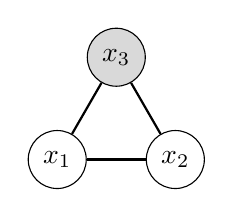
\begin{tikzpicture}
        \node[style=visible] (a) at (0, 0) {$x_{1}$};
        \node[style=visible] (b) at +(0: 1.5) {$x_{2}$};
        \node[style=hidden] (c) at + (60: 1.5) {$x_{3}$};
        \foreach \from/\to in {a/b, b/c, c/a}
            \draw [thick] (\from) -- (\to);   
    \end{tikzpicture}
  	\legend{Gray circles represent the hidden units of the Boltzmann Machine, while the white circles are the visible units.}
    % \source{\license}
\end{figure}